\documentclass{prova}

\usepackage{amsmath}
\usepackage{amsfonts}

\setlength{\textheight}{25cm}

\renewcommand{\sin}{\,\mbox{sen}\,}
\newcommand{\ds}{\displaystyle}

\professor{Prof.\@ Adriano Barbosa}
\disciplina{C\'alculo de V\'arias Vari\'aveis}
\avaliacao{P1}
\curso{Matem\'atica}
\data{12/07/2023}

\begin{document}
	\cabecalho{5}  % o numero 5 indica a qnt de quadros na tabela de nota

    \textbf{Todas as respostas devem ser justificadas.}

    \begin{questionario}
        \q{Esboce o maior dom\'{\i}nio das fun\c{c}\~oes abaixo ou descreva-os com
           suas palavras.}
            \begin{questionario}
                \qq{$f(x,y) = \sqrt{1-x^2} - \sqrt{1-y^2}$}
                \qq{$f(x,y,z) = \sqrt{1-x^2-y^2-z^2}$}
            \end{questionario}
        \q{Seja $f$ \'e diferenci\'avel com $f(2,5)=3$, $\frac{\partial
           f}{\partial x}(2,5)=-1$ e $\frac{\partial f}{\partial y}(2,5)=1$,
           utilize a aproxima\c{c}\~ao linear de $f$ em $(2,5)$ para estimar o valor de
           $f(2.1, 4.9)$.}
        \q{Seja $z=f(x,y)$, onde $x=r\cos(\theta)$ e $y=r\sin(\theta)$. Calcule
           $\ds\frac{\partial^2 z}{\partial r\partial\theta}$.}
        \q{Determine a taxa de varia\c{c}\~ao m\'axima de $f(x,y)=x^2+y^2-2x-4y$ em
           $(0,0)$ e a dire\c{c}\~ao em que ela ocorre.}

        %\q{Um pent\'agono \'e formato utilizando um tri\^angulo isosceles e um
        %   ret\^angulo como na figura abaixo. Se o pent\'agono tem per\'{\i}metro $P$ fixo,
        %   determine o comprimento dos lados do pent\'agono que tem a maior \'area
        %   poss\'{\i}vel.}
        %   \begin{figure}[h]
        %       \centering
        %       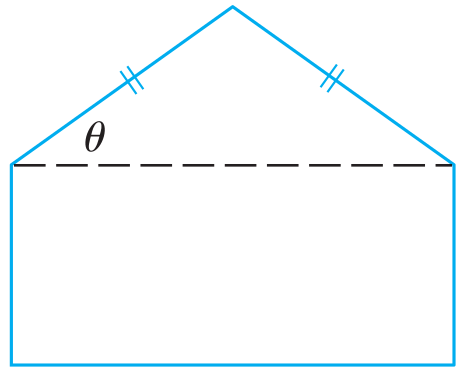
\includegraphics[width=0.25\textwidth]{fig1.png}
        %   \end{figure}
        \q{Um ret\^angulo de largura $L$ e altura $H$ \'e cortado em quatro
           ret\^angulos menores por duas linhas perpendiculares entre si e paralelas
           a seus lados. Encontre o valor m\'{\i}nimo para a soma dos quadrados das
           \'areas dos ret\^angulos menores.}
           (Dica: simplifique $f$ antes de calcular as derivadas.)
           \begin{figure}[h]
               \centering
               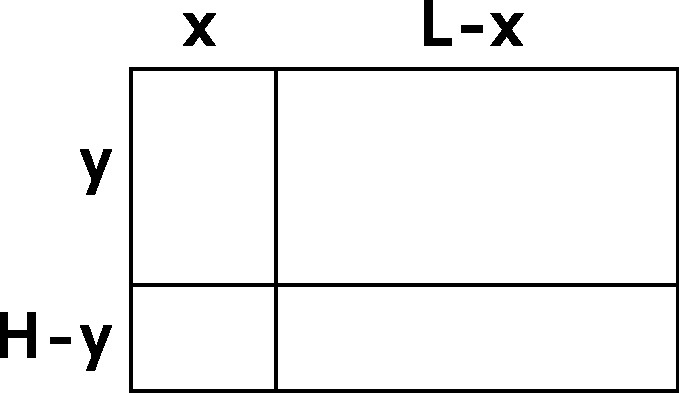
\includegraphics[width=0.25\textwidth]{fig1.pdf}
           \end{figure}
    \end{questionario}
\end{document}
